% Options for packages loaded elsewhere
\PassOptionsToPackage{unicode}{hyperref}
\PassOptionsToPackage{hyphens}{url}
%
\documentclass[
]{article}
\usepackage{amsmath,amssymb}
\usepackage{lmodern}
\usepackage{iftex}
\ifPDFTeX
  \usepackage[T1]{fontenc}
  \usepackage[utf8]{inputenc}
  \usepackage{textcomp} % provide euro and other symbols
\else % if luatex or xetex
  \usepackage{unicode-math}
  \defaultfontfeatures{Scale=MatchLowercase}
  \defaultfontfeatures[\rmfamily]{Ligatures=TeX,Scale=1}
\fi
% Use upquote if available, for straight quotes in verbatim environments
\IfFileExists{upquote.sty}{\usepackage{upquote}}{}
\IfFileExists{microtype.sty}{% use microtype if available
  \usepackage[]{microtype}
  \UseMicrotypeSet[protrusion]{basicmath} % disable protrusion for tt fonts
}{}
\makeatletter
\@ifundefined{KOMAClassName}{% if non-KOMA class
  \IfFileExists{parskip.sty}{%
    \usepackage{parskip}
  }{% else
    \setlength{\parindent}{0pt}
    \setlength{\parskip}{6pt plus 2pt minus 1pt}}
}{% if KOMA class
  \KOMAoptions{parskip=half}}
\makeatother
\usepackage{xcolor}
\IfFileExists{xurl.sty}{\usepackage{xurl}}{} % add URL line breaks if available
\IfFileExists{bookmark.sty}{\usepackage{bookmark}}{\usepackage{hyperref}}
\hypersetup{
  pdftitle={Midterm Exam: Preston Robertson},
  hidelinks,
  pdfcreator={LaTeX via pandoc}}
\urlstyle{same} % disable monospaced font for URLs
\usepackage[margin=1in]{geometry}
\usepackage{color}
\usepackage{fancyvrb}
\newcommand{\VerbBar}{|}
\newcommand{\VERB}{\Verb[commandchars=\\\{\}]}
\DefineVerbatimEnvironment{Highlighting}{Verbatim}{commandchars=\\\{\}}
% Add ',fontsize=\small' for more characters per line
\usepackage{framed}
\definecolor{shadecolor}{RGB}{248,248,248}
\newenvironment{Shaded}{\begin{snugshade}}{\end{snugshade}}
\newcommand{\AlertTok}[1]{\textcolor[rgb]{0.94,0.16,0.16}{#1}}
\newcommand{\AnnotationTok}[1]{\textcolor[rgb]{0.56,0.35,0.01}{\textbf{\textit{#1}}}}
\newcommand{\AttributeTok}[1]{\textcolor[rgb]{0.77,0.63,0.00}{#1}}
\newcommand{\BaseNTok}[1]{\textcolor[rgb]{0.00,0.00,0.81}{#1}}
\newcommand{\BuiltInTok}[1]{#1}
\newcommand{\CharTok}[1]{\textcolor[rgb]{0.31,0.60,0.02}{#1}}
\newcommand{\CommentTok}[1]{\textcolor[rgb]{0.56,0.35,0.01}{\textit{#1}}}
\newcommand{\CommentVarTok}[1]{\textcolor[rgb]{0.56,0.35,0.01}{\textbf{\textit{#1}}}}
\newcommand{\ConstantTok}[1]{\textcolor[rgb]{0.00,0.00,0.00}{#1}}
\newcommand{\ControlFlowTok}[1]{\textcolor[rgb]{0.13,0.29,0.53}{\textbf{#1}}}
\newcommand{\DataTypeTok}[1]{\textcolor[rgb]{0.13,0.29,0.53}{#1}}
\newcommand{\DecValTok}[1]{\textcolor[rgb]{0.00,0.00,0.81}{#1}}
\newcommand{\DocumentationTok}[1]{\textcolor[rgb]{0.56,0.35,0.01}{\textbf{\textit{#1}}}}
\newcommand{\ErrorTok}[1]{\textcolor[rgb]{0.64,0.00,0.00}{\textbf{#1}}}
\newcommand{\ExtensionTok}[1]{#1}
\newcommand{\FloatTok}[1]{\textcolor[rgb]{0.00,0.00,0.81}{#1}}
\newcommand{\FunctionTok}[1]{\textcolor[rgb]{0.00,0.00,0.00}{#1}}
\newcommand{\ImportTok}[1]{#1}
\newcommand{\InformationTok}[1]{\textcolor[rgb]{0.56,0.35,0.01}{\textbf{\textit{#1}}}}
\newcommand{\KeywordTok}[1]{\textcolor[rgb]{0.13,0.29,0.53}{\textbf{#1}}}
\newcommand{\NormalTok}[1]{#1}
\newcommand{\OperatorTok}[1]{\textcolor[rgb]{0.81,0.36,0.00}{\textbf{#1}}}
\newcommand{\OtherTok}[1]{\textcolor[rgb]{0.56,0.35,0.01}{#1}}
\newcommand{\PreprocessorTok}[1]{\textcolor[rgb]{0.56,0.35,0.01}{\textit{#1}}}
\newcommand{\RegionMarkerTok}[1]{#1}
\newcommand{\SpecialCharTok}[1]{\textcolor[rgb]{0.00,0.00,0.00}{#1}}
\newcommand{\SpecialStringTok}[1]{\textcolor[rgb]{0.31,0.60,0.02}{#1}}
\newcommand{\StringTok}[1]{\textcolor[rgb]{0.31,0.60,0.02}{#1}}
\newcommand{\VariableTok}[1]{\textcolor[rgb]{0.00,0.00,0.00}{#1}}
\newcommand{\VerbatimStringTok}[1]{\textcolor[rgb]{0.31,0.60,0.02}{#1}}
\newcommand{\WarningTok}[1]{\textcolor[rgb]{0.56,0.35,0.01}{\textbf{\textit{#1}}}}
\usepackage{graphicx}
\makeatletter
\def\maxwidth{\ifdim\Gin@nat@width>\linewidth\linewidth\else\Gin@nat@width\fi}
\def\maxheight{\ifdim\Gin@nat@height>\textheight\textheight\else\Gin@nat@height\fi}
\makeatother
% Scale images if necessary, so that they will not overflow the page
% margins by default, and it is still possible to overwrite the defaults
% using explicit options in \includegraphics[width, height, ...]{}
\setkeys{Gin}{width=\maxwidth,height=\maxheight,keepaspectratio}
% Set default figure placement to htbp
\makeatletter
\def\fps@figure{htbp}
\makeatother
\setlength{\emergencystretch}{3em} % prevent overfull lines
\providecommand{\tightlist}{%
  \setlength{\itemsep}{0pt}\setlength{\parskip}{0pt}}
\setcounter{secnumdepth}{-\maxdimen} % remove section numbering
\ifLuaTeX
  \usepackage{selnolig}  % disable illegal ligatures
\fi

\title{Midterm Exam: Preston Robertson}
\author{}
\date{\vspace{-2.5em}}

\begin{document}
\maketitle

\begin{Shaded}
\begin{Highlighting}[]
\CommentTok{\# Fixing the flights data}

\NormalTok{make\_datetime\_100 }\OtherTok{\textless{}{-}} \ControlFlowTok{function}\NormalTok{(year, month, day, time) \{}
  \FunctionTok{make\_datetime}\NormalTok{(year, month, day, time }\SpecialCharTok{\%/\%} \DecValTok{100}\NormalTok{, time }\SpecialCharTok{\%\%} \DecValTok{100}\NormalTok{)}
\NormalTok{\}}


\NormalTok{flights\_fixed }\OtherTok{\textless{}{-}}\NormalTok{ flights }\SpecialCharTok{\%\textgreater{}\%}
  \FunctionTok{filter}\NormalTok{(}\SpecialCharTok{!}\FunctionTok{is.na}\NormalTok{(dep\_time), }\SpecialCharTok{!}\FunctionTok{is.na}\NormalTok{(arr\_time)) }\SpecialCharTok{\%\textgreater{}\%}
  \FunctionTok{mutate}\NormalTok{(}
    \AttributeTok{dep\_time =} \FunctionTok{make\_datetime\_100}\NormalTok{(year, month, day, dep\_time),}
    \AttributeTok{arr\_time =} \FunctionTok{make\_datetime\_100}\NormalTok{(year, month, day, arr\_time),}
    \AttributeTok{sched\_dep\_time =} \FunctionTok{make\_datetime\_100}\NormalTok{(year, month, day, sched\_dep\_time),}
    \AttributeTok{sched\_arr\_time =} \FunctionTok{make\_datetime\_100}\NormalTok{(year, month, day, sched\_arr\_time)}
\NormalTok{  ) }\SpecialCharTok{\%\textgreater{}\%}
  \FunctionTok{select}\NormalTok{(origin, dest, }\FunctionTok{ends\_with}\NormalTok{(}\StringTok{"delay"}\NormalTok{), }\FunctionTok{ends\_with}\NormalTok{(}\StringTok{"time"}\NormalTok{))}
\end{Highlighting}
\end{Shaded}

All of these problems are from the \emph{R for Data Science} book. The
section numbers (e.g., ``3.2.4 Exercises'') refer to sections in this
book.

When solving these problems, you are allowed to use any method from the
book or class, even if that method wasn't yet covered when the exercise
was presented in the book.

Because this is an exam, you need to do the work by yourself. Do not
collaborate on this exam.

This exam is out of 60 points.

\begin{center}\rule{0.5\linewidth}{0.5pt}\end{center}

\hypertarget{exercises}{%
\subsection{12.2.1 Exercises}\label{exercises}}

\hypertarget{exercise-2-10-pts}{%
\subsubsection{(1) 12.2.1 Exercise 2 (10 pts)}\label{exercise-2-10-pts}}

Compute the \texttt{rate} for \texttt{table2}, and \texttt{table4a} +
\texttt{table4b}. You will need to perform four operations :

\begin{Shaded}
\begin{Highlighting}[]
\NormalTok{table1}
\end{Highlighting}
\end{Shaded}

\begin{verbatim}
# A tibble: 6 x 4
  country      year  cases population
  <chr>       <int>  <int>      <int>
1 Afghanistan  1999    745   19987071
2 Afghanistan  2000   2666   20595360
3 Brazil       1999  37737  172006362
4 Brazil       2000  80488  174504898
5 China        1999 212258 1272915272
6 China        2000 213766 1280428583
\end{verbatim}

\begin{Shaded}
\begin{Highlighting}[]
\NormalTok{table2 }\CommentTok{\#Cases and Population are in separate rows}
\end{Highlighting}
\end{Shaded}

\begin{verbatim}
# A tibble: 12 x 4
   country      year type            count
   <chr>       <int> <chr>           <int>
 1 Afghanistan  1999 cases             745
 2 Afghanistan  1999 population   19987071
 3 Afghanistan  2000 cases            2666
 4 Afghanistan  2000 population   20595360
 5 Brazil       1999 cases           37737
 6 Brazil       1999 population  172006362
 7 Brazil       2000 cases           80488
 8 Brazil       2000 population  174504898
 9 China        1999 cases          212258
10 China        1999 population 1272915272
11 China        2000 cases          213766
12 China        2000 population 1280428583
\end{verbatim}

\begin{Shaded}
\begin{Highlighting}[]
\NormalTok{table3}
\end{Highlighting}
\end{Shaded}

\begin{verbatim}
# A tibble: 6 x 3
  country      year rate             
* <chr>       <int> <chr>            
1 Afghanistan  1999 745/19987071     
2 Afghanistan  2000 2666/20595360    
3 Brazil       1999 37737/172006362  
4 Brazil       2000 80488/174504898  
5 China        1999 212258/1272915272
6 China        2000 213766/1280428583
\end{verbatim}

\begin{Shaded}
\begin{Highlighting}[]
\NormalTok{table4a }\CommentTok{\# Cases and Population are in different tables}
\end{Highlighting}
\end{Shaded}

\begin{verbatim}
# A tibble: 3 x 3
  country     `1999` `2000`
* <chr>        <int>  <int>
1 Afghanistan    745   2666
2 Brazil       37737  80488
3 China       212258 213766
\end{verbatim}

\begin{Shaded}
\begin{Highlighting}[]
\NormalTok{table4b}
\end{Highlighting}
\end{Shaded}

\begin{verbatim}
# A tibble: 3 x 3
  country         `1999`     `2000`
* <chr>            <int>      <int>
1 Afghanistan   19987071   20595360
2 Brazil       172006362  174504898
3 China       1272915272 1280428583
\end{verbatim}

\begin{enumerate}
\def\labelenumi{\arabic{enumi}.}
\item
  Extract the number of TB cases per country per year.
\item
  Extract the matching population per country per year.
\item
  Divide cases by population, and multiply by 1000.
\item
  Store back in the appropriate place.
\end{enumerate}

Which representation is easiest to work with? Which is hardest? Why?

\begin{Shaded}
\begin{Highlighting}[]
\CommentTok{\# Table 2}

\CommentTok{\# First step take out old values (parts 1 and 2)}
\NormalTok{t2\_case }\OtherTok{\textless{}{-}} \FunctionTok{filter}\NormalTok{(table2, type }\SpecialCharTok{==} \StringTok{"cases"}\NormalTok{) }\SpecialCharTok{\%\textgreater{}\%}
  \FunctionTok{rename}\NormalTok{(}\AttributeTok{cases =}\NormalTok{ count) }\SpecialCharTok{\%\textgreater{}\%}
  \FunctionTok{arrange}\NormalTok{(country, year) }\CommentTok{\# Keeping order}
\NormalTok{t2\_pop }\OtherTok{\textless{}{-}} \FunctionTok{filter}\NormalTok{(table2, type }\SpecialCharTok{==} \StringTok{"population"}\NormalTok{) }\SpecialCharTok{\%\textgreater{}\%}
  \FunctionTok{rename}\NormalTok{(}\AttributeTok{population =}\NormalTok{ count) }\SpecialCharTok{\%\textgreater{}\%}
  \FunctionTok{arrange}\NormalTok{(country, year)}

\CommentTok{\# Step 2 calculate the rate}
\NormalTok{t2\_rate }\OtherTok{\textless{}{-}} \FunctionTok{tibble}\NormalTok{(}\AttributeTok{year =}\NormalTok{ t2\_case}\SpecialCharTok{$}\NormalTok{year, }\AttributeTok{country =}\NormalTok{ t2\_case}\SpecialCharTok{$}\NormalTok{country,}\AttributeTok{cases =}\NormalTok{ t2\_case}\SpecialCharTok{$}\NormalTok{cases,}
                  \AttributeTok{population =}\NormalTok{ t2\_pop}\SpecialCharTok{$}\NormalTok{population) }\SpecialCharTok{\%\textgreater{}\%}
  \FunctionTok{mutate}\NormalTok{(}\AttributeTok{rate =}\NormalTok{ (cases }\SpecialCharTok{/}\NormalTok{ population) }\SpecialCharTok{*} \DecValTok{1000}\NormalTok{) }\SpecialCharTok{\%\textgreater{}\%} \CommentTok{\#Doing part 3}
  \FunctionTok{select}\NormalTok{(country, year, rate)}

\CommentTok{\# Step 3 Combine the rate with table 2}
\NormalTok{t2\_rate }\OtherTok{\textless{}{-}}\NormalTok{ t2\_rate }\SpecialCharTok{\%\textgreater{}\%}
  \FunctionTok{mutate}\NormalTok{(}\AttributeTok{type =} \StringTok{"rate"}\NormalTok{) }\SpecialCharTok{\%\textgreater{}\%}
  \FunctionTok{rename}\NormalTok{(}\AttributeTok{count =}\NormalTok{ rate) }\CommentTok{\#So rate will go to the proper column}
\FunctionTok{bind\_rows}\NormalTok{(table2, t2\_rate) }\SpecialCharTok{\%\textgreater{}\%}
  \FunctionTok{arrange}\NormalTok{(country, year, type, count)}
\end{Highlighting}
\end{Shaded}

\begin{verbatim}
# A tibble: 18 x 4
   country      year type         count
   <chr>       <int> <chr>        <dbl>
 1 Afghanistan  1999 cases      7.45e+2
 2 Afghanistan  1999 population 2.00e+7
 3 Afghanistan  1999 rate       3.73e-2
 4 Afghanistan  2000 cases      2.67e+3
 5 Afghanistan  2000 population 2.06e+7
 6 Afghanistan  2000 rate       1.29e-1
 7 Brazil       1999 cases      3.77e+4
 8 Brazil       1999 population 1.72e+8
 9 Brazil       1999 rate       2.19e-1
10 Brazil       2000 cases      8.05e+4
11 Brazil       2000 population 1.75e+8
12 Brazil       2000 rate       4.61e-1
13 China        1999 cases      2.12e+5
14 China        1999 population 1.27e+9
15 China        1999 rate       1.67e-1
16 China        2000 cases      2.14e+5
17 China        2000 population 1.28e+9
18 China        2000 rate       1.67e-1
\end{verbatim}

\begin{Shaded}
\begin{Highlighting}[]
\NormalTok{table2}
\end{Highlighting}
\end{Shaded}

\begin{verbatim}
# A tibble: 12 x 4
   country      year type            count
   <chr>       <int> <chr>           <int>
 1 Afghanistan  1999 cases             745
 2 Afghanistan  1999 population   19987071
 3 Afghanistan  2000 cases            2666
 4 Afghanistan  2000 population   20595360
 5 Brazil       1999 cases           37737
 6 Brazil       1999 population  172006362
 7 Brazil       2000 cases           80488
 8 Brazil       2000 population  174504898
 9 China        1999 cases          212258
10 China        1999 population 1272915272
11 China        2000 cases          213766
12 China        2000 population 1280428583
\end{verbatim}

\begin{Shaded}
\begin{Highlighting}[]
\CommentTok{\# Table 4}

\CommentTok{\# Table 4 is already split so just make a new table and skip step 1 and step 3 above}
\NormalTok{table4 }\OtherTok{\textless{}{-}} \FunctionTok{tibble}\NormalTok{(}
    \AttributeTok{country =}\NormalTok{ table4a}\SpecialCharTok{$}\NormalTok{country,}
    \StringTok{\textasciigrave{}}\AttributeTok{1999}\StringTok{\textasciigrave{}} \OtherTok{=}\NormalTok{ table4a[[}\StringTok{"1999"}\NormalTok{]] }\SpecialCharTok{/}\NormalTok{ table4b[[}\StringTok{"1999"}\NormalTok{]] }\SpecialCharTok{*} \DecValTok{1000}\NormalTok{, }\CommentTok{\# First value is table cases of 1999 and second is population of \textasciigrave{}1999}
    \StringTok{\textasciigrave{}}\AttributeTok{2000}\StringTok{\textasciigrave{}} \OtherTok{=}\NormalTok{ table4a[[}\StringTok{"2000"}\NormalTok{]] }\SpecialCharTok{/}\NormalTok{ table4b[[}\StringTok{"2000"}\NormalTok{]] }\SpecialCharTok{*} \DecValTok{1000}
\NormalTok{  )}

\NormalTok{table4}
\end{Highlighting}
\end{Shaded}

\begin{verbatim}
# A tibble: 3 x 3
  country     `1999` `2000`
  <chr>        <dbl>  <dbl>
1 Afghanistan 0.0373  0.129
2 Brazil      0.219   0.461
3 China       0.167   0.167
\end{verbatim}

\begin{Shaded}
\begin{Highlighting}[]
\CommentTok{\# Which is harder to work with? Easily table2 for me. The data sets that I normally work with do not work like a branching system where the previous columns work as dictionaries for the value column. It took me forever to think to take out the values and then do the math. It also was difficult to find out to plug them back in, I had to "jerry{-}rig" by just saying rate is count. Table4 allowed for simple operations already plugged into r. It is still inconvenient to call multiple different tables, but way more manageable than table2 for me.}
\end{Highlighting}
\end{Shaded}

\hypertarget{exercises-1}{%
\subsection{12.3.3 Exercises}\label{exercises-1}}

\hypertarget{exercise-1-10-pts}{%
\subsubsection{(2) 12.3.3 Exercise 1 (10 pts)}\label{exercise-1-10-pts}}

Why are \texttt{pivot\_longer()} and \texttt{pivot\_wider()} not
perfectly symmetrical? Carefully consider the following example:

(Hint: look at the variable types and think about column \emph{names}.)
\texttt{pivot\_longer()} has a \texttt{names\_transform} argument. What
does it do?

\begin{Shaded}
\begin{Highlighting}[]
\NormalTok{stocks }\OtherTok{\textless{}{-}} \FunctionTok{tibble}\NormalTok{(}
  \AttributeTok{year   =} \FunctionTok{c}\NormalTok{(}\DecValTok{2015}\NormalTok{, }\DecValTok{2015}\NormalTok{, }\DecValTok{2016}\NormalTok{, }\DecValTok{2016}\NormalTok{),}
  \AttributeTok{half  =} \FunctionTok{c}\NormalTok{(   }\DecValTok{1}\NormalTok{,    }\DecValTok{2}\NormalTok{,     }\DecValTok{1}\NormalTok{,    }\DecValTok{2}\NormalTok{),}
  \AttributeTok{return =} \FunctionTok{c}\NormalTok{(}\FloatTok{1.88}\NormalTok{, }\FloatTok{0.59}\NormalTok{, }\FloatTok{0.92}\NormalTok{, }\FloatTok{0.17}\NormalTok{)}
\NormalTok{)}

\NormalTok{stocks}
\end{Highlighting}
\end{Shaded}

\begin{verbatim}
# A tibble: 4 x 3
   year  half return
  <dbl> <dbl>  <dbl>
1  2015     1   1.88
2  2015     2   0.59
3  2016     1   0.92
4  2016     2   0.17
\end{verbatim}

\begin{Shaded}
\begin{Highlighting}[]
\NormalTok{stocks\_wrong }\OtherTok{\textless{}{-}}\NormalTok{ stocks }\SpecialCharTok{\%\textgreater{}\%} 
  \FunctionTok{pivot\_wider}\NormalTok{(}\AttributeTok{names\_from =}\NormalTok{ year, }\AttributeTok{values\_from =}\NormalTok{ return) }\SpecialCharTok{\%\textgreater{}\%} 
  \FunctionTok{pivot\_longer}\NormalTok{(}\StringTok{\textasciigrave{}}\AttributeTok{2015}\StringTok{\textasciigrave{}}\SpecialCharTok{:}\StringTok{\textasciigrave{}}\AttributeTok{2016}\StringTok{\textasciigrave{}}\NormalTok{, }\AttributeTok{names\_to =} \StringTok{"year"}\NormalTok{, }\AttributeTok{values\_to =} \StringTok{"return"}\NormalTok{)}

\NormalTok{stocks\_wrong}
\end{Highlighting}
\end{Shaded}

\begin{verbatim}
# A tibble: 4 x 3
   half year  return
  <dbl> <chr>  <dbl>
1     1 2015    1.88
2     1 2016    0.92
3     2 2015    0.59
4     2 2016    0.17
\end{verbatim}

\begin{Shaded}
\begin{Highlighting}[]
\CommentTok{\# The pivot\_longer() function turned the year column from a numeric value (double) to a character value. This is because the \textquotesingle{}names\_to\textquotesingle{} function inside pivot\_longer assumes all values to be a character. }

\CommentTok{\# The \textquotesingle{}names\_transform\textquotesingle{} argument allows the user to change the character type from the \textquotesingle{}names\_to\textquotesingle{} argument back to a numeric data type.}

\NormalTok{stocks }\SpecialCharTok{\%\textgreater{}\%}
  \FunctionTok{pivot\_wider}\NormalTok{(}\AttributeTok{names\_from =}\NormalTok{ year, }\AttributeTok{values\_from =}\NormalTok{ return)}\SpecialCharTok{\%\textgreater{}\%}
  \FunctionTok{pivot\_longer}\NormalTok{(}\StringTok{\textasciigrave{}}\AttributeTok{2015}\StringTok{\textasciigrave{}}\SpecialCharTok{:}\StringTok{\textasciigrave{}}\AttributeTok{2016}\StringTok{\textasciigrave{}}\NormalTok{, }\AttributeTok{names\_to =} \StringTok{"year"}\NormalTok{, }\AttributeTok{values\_to =} \StringTok{"return"}\NormalTok{, }\AttributeTok{names\_transform =} \FunctionTok{list}\NormalTok{(}\AttributeTok{year =}\NormalTok{ as.numeric))}
\end{Highlighting}
\end{Shaded}

\begin{verbatim}
# A tibble: 4 x 3
   half  year return
  <dbl> <dbl>  <dbl>
1     1  2015   1.88
2     1  2016   0.92
3     2  2015   0.59
4     2  2016   0.17
\end{verbatim}

\hypertarget{exercises-2}{%
\subsection{16.3.4 Exercises}\label{exercises-2}}

\hypertarget{exercise-2-10-pts-1}{%
\subsubsection{(3) 16.3.4 Exercise 2 (10
pts)}\label{exercise-2-10-pts-1}}

Compare \texttt{dep\_time}, \texttt{sched\_dep\_time} and
\texttt{dep\_delay}. I recommend looking at the distributions over an
hour. Are they consistent? Explain your findings.

\begin{Shaded}
\begin{Highlighting}[]
\NormalTok{Question3}\FloatTok{.1} \OtherTok{\textless{}{-}}\NormalTok{ flights\_fixed }\SpecialCharTok{\%\textgreater{}\%} \FunctionTok{select}\NormalTok{(}\FunctionTok{contains}\NormalTok{(}\StringTok{\textquotesingle{}dep\textquotesingle{}}\NormalTok{)) }\SpecialCharTok{\%\textgreater{}\%}
  \FunctionTok{mutate}\NormalTok{(}\AttributeTok{calculated\_delay =} \FunctionTok{as.numeric}\NormalTok{(dep\_time }\SpecialCharTok{{-}}\NormalTok{ sched\_dep\_time) }\SpecialCharTok{/} \DecValTok{60}\NormalTok{) }\SpecialCharTok{\%\textgreater{}\%} \CommentTok{\#Calculating departure delay manually}
  \FunctionTok{filter}\NormalTok{(dep\_delay }\SpecialCharTok{!=}\NormalTok{ calculated\_delay) }\CommentTok{\#Filtering all the inconsistencies}

\NormalTok{Question3}\FloatTok{.1}
\end{Highlighting}
\end{Shaded}

\begin{verbatim}
# A tibble: 1,205 x 4
   dep_delay dep_time            sched_dep_time      calculated_delay
       <dbl> <dttm>              <dttm>                         <dbl>
 1       853 2013-01-01 08:48:00 2013-01-01 18:35:00             -587
 2        43 2013-01-02 00:42:00 2013-01-02 23:59:00            -1397
 3       156 2013-01-02 01:26:00 2013-01-02 22:50:00            -1284
 4        33 2013-01-03 00:32:00 2013-01-03 23:59:00            -1407
 5       185 2013-01-03 00:50:00 2013-01-03 21:45:00            -1255
 6       156 2013-01-03 02:35:00 2013-01-03 23:59:00            -1284
 7        26 2013-01-04 00:25:00 2013-01-04 23:59:00            -1414
 8       141 2013-01-04 01:06:00 2013-01-04 22:45:00            -1299
 9        15 2013-01-05 00:14:00 2013-01-05 23:59:00            -1425
10       127 2013-01-05 00:37:00 2013-01-05 22:30:00            -1313
# ... with 1,195 more rows
\end{verbatim}

\begin{Shaded}
\begin{Highlighting}[]
\NormalTok{flights\_fixed }\SpecialCharTok{\%\textgreater{}\%} \FunctionTok{select}\NormalTok{(}\FunctionTok{contains}\NormalTok{(}\StringTok{\textquotesingle{}dep\textquotesingle{}}\NormalTok{)) }\SpecialCharTok{\%\textgreater{}\%}
  \FunctionTok{mutate}\NormalTok{(}\AttributeTok{cal\_delay =} \FunctionTok{as.numeric}\NormalTok{(dep\_time }\SpecialCharTok{{-}}\NormalTok{ sched\_dep\_time) }\SpecialCharTok{/} \DecValTok{60}\NormalTok{) }\SpecialCharTok{\%\textgreater{}\%}
  \FunctionTok{filter}\NormalTok{(dep\_delay }\SpecialCharTok{!=}\NormalTok{ cal\_delay) }\SpecialCharTok{\%\textgreater{}\%}
  \FunctionTok{mutate}\NormalTok{(}\AttributeTok{dep\_time =} \FunctionTok{update}\NormalTok{(dep\_time, }\AttributeTok{mday =} \FunctionTok{mday}\NormalTok{(dep\_time) }\SpecialCharTok{+} \DecValTok{1}\NormalTok{)) }\SpecialCharTok{\%\textgreater{}\%} \CommentTok{\#Adding one day to all of the previous table}
  \FunctionTok{mutate}\NormalTok{(}\AttributeTok{cal\_delay =} \FunctionTok{as.numeric}\NormalTok{(dep\_time }\SpecialCharTok{{-}}\NormalTok{ sched\_dep\_time)) }\SpecialCharTok{\%\textgreater{}\%} \CommentTok{\# Re{-}doing above process}
  \FunctionTok{filter}\NormalTok{(dep\_delay }\SpecialCharTok{!=}\NormalTok{ cal\_delay)}
\end{Highlighting}
\end{Shaded}

\begin{verbatim}
# A tibble: 0 x 4
# ... with 4 variables: dep_delay <dbl>, dep_time <dttm>,
#   sched_dep_time <dttm>, cal_delay <dbl>
\end{verbatim}

\begin{Shaded}
\begin{Highlighting}[]
\CommentTok{\# Looking at the below table, you can see that the calculated delay shows that some flights actually leave earlier and were not delayed. However that was probably a mistake on the people recording the flights. To fix this we are going to add a day onto negative values}
\end{Highlighting}
\end{Shaded}

\hypertarget{exercise-4-10-pts}{%
\subsubsection{(4) 16.3.4 Exercise 4 (10 pts)}\label{exercise-4-10-pts}}

How does the average departure delay change over the course of a day?
Should you use \texttt{dep\_time} or \texttt{sched\_dep\_time}? Why?

\begin{Shaded}
\begin{Highlighting}[]
\CommentTok{\# We should you scheduled departure time since that is what the delay is based on.}
\CommentTok{\# Looking at the graph, we can see a clear trend that the farther the day goes until around 7pm the delays add up. The delays are probably due to a mix of busyness during those times, plus other flights being delayed have a ripple effect on the airport.}

\NormalTok{flights\_fixed }\SpecialCharTok{\%\textgreater{}\%}
  \FunctionTok{mutate}\NormalTok{(}\AttributeTok{hour =} \FunctionTok{hour}\NormalTok{(sched\_dep\_time)) }\SpecialCharTok{\%\textgreater{}\%}
  \FunctionTok{group\_by}\NormalTok{(hour) }\SpecialCharTok{\%\textgreater{}\%}
  \FunctionTok{summarize}\NormalTok{(}\AttributeTok{avg\_dep\_delay =} \FunctionTok{mean}\NormalTok{(dep\_delay)) }\SpecialCharTok{\%\textgreater{}\%}
  \FunctionTok{ggplot}\NormalTok{(}\AttributeTok{mapping =} \FunctionTok{aes}\NormalTok{(}\AttributeTok{x =}\NormalTok{ hour, }\AttributeTok{y =}\NormalTok{ avg\_dep\_delay)) }\SpecialCharTok{+}
  \FunctionTok{geom\_smooth}\NormalTok{() }\SpecialCharTok{+}
  \FunctionTok{labs}\NormalTok{(}\AttributeTok{y =} \StringTok{"Depature Delay"}\NormalTok{, }\AttributeTok{x =} \StringTok{"Hour"}\NormalTok{)}
\end{Highlighting}
\end{Shaded}

\begin{verbatim}
`geom_smooth()` using method = 'loess' and formula 'y ~ x'
\end{verbatim}

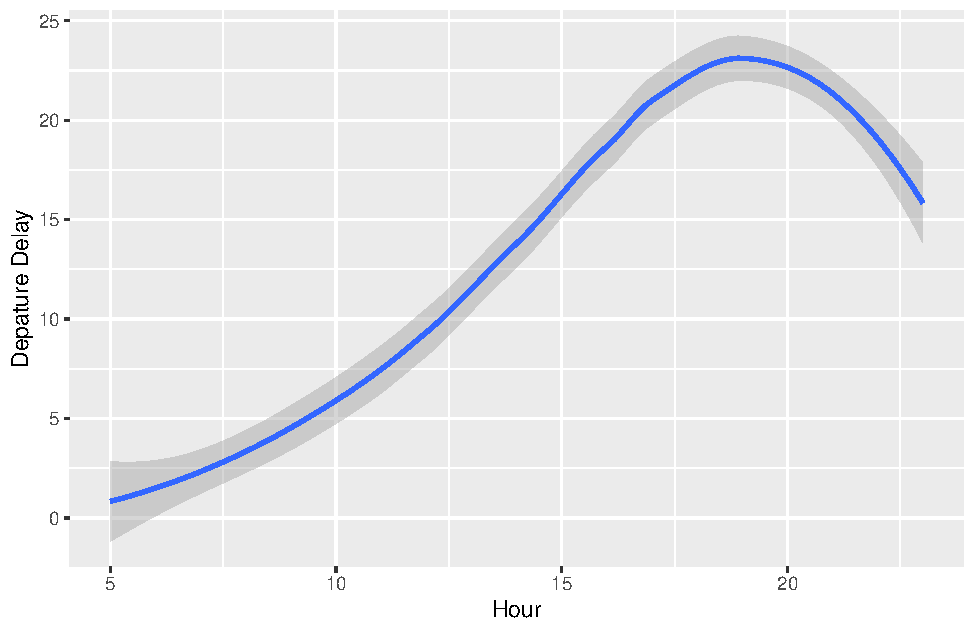
\includegraphics{Midterm.sa_files/figure-latex/unnamed-chunk-6-1.pdf}

\hypertarget{exercise-5-10-pts}{%
\subsubsection{(5) 16.3.4 Exercise 5 (10 pts)}\label{exercise-5-10-pts}}

On what day of the week should you leave if you want to minimize the
chance of a departure delay?

\begin{Shaded}
\begin{Highlighting}[]
\NormalTok{flights\_days }\OtherTok{\textless{}{-}}\NormalTok{ flights\_fixed }\SpecialCharTok{\%\textgreater{}\%}
  \FunctionTok{mutate}\NormalTok{(}\AttributeTok{days =} \FunctionTok{wday}\NormalTok{(sched\_dep\_time)) }\SpecialCharTok{\%\textgreater{}\%} \CommentTok{\# Grouping into day of the week, Sunday is 1}
  \FunctionTok{group\_by}\NormalTok{(days) }\SpecialCharTok{\%\textgreater{}\%}
  \FunctionTok{summarise}\NormalTok{(}
    \AttributeTok{dep\_delay =} \FunctionTok{mean}\NormalTok{(dep\_delay), }\CommentTok{\#Averaging all values into a single one.}
    \AttributeTok{arr\_delay =} \FunctionTok{mean}\NormalTok{(arr\_delay, }\AttributeTok{na.rm =} \ConstantTok{TRUE}\NormalTok{)}
\NormalTok{  ) }


  
\FunctionTok{ggplot}\NormalTok{(flights\_days) }\SpecialCharTok{+}
  \FunctionTok{geom\_point}\NormalTok{(}\AttributeTok{mapping =} \FunctionTok{aes}\NormalTok{(}\AttributeTok{x =}\NormalTok{ days, }\AttributeTok{y =}\NormalTok{ dep\_delay, }\AttributeTok{colour =} \StringTok{"red"}\NormalTok{)) }\SpecialCharTok{+}
  \FunctionTok{geom\_smooth}\NormalTok{(}\AttributeTok{mapping =} \FunctionTok{aes}\NormalTok{(}\AttributeTok{x =}\NormalTok{ days, }\AttributeTok{y =}\NormalTok{ dep\_delay, }\AttributeTok{colour =} \StringTok{"red"}\NormalTok{)) }\SpecialCharTok{+}
  \FunctionTok{geom\_point}\NormalTok{(}\AttributeTok{mapping =} \FunctionTok{aes}\NormalTok{(}\AttributeTok{x =}\NormalTok{ days, }\AttributeTok{y =}\NormalTok{ arr\_delay, }\AttributeTok{colour =} \StringTok{"blue"}\NormalTok{)) }\SpecialCharTok{+}
  \FunctionTok{geom\_smooth}\NormalTok{(}\AttributeTok{mapping =} \FunctionTok{aes}\NormalTok{(}\AttributeTok{x =}\NormalTok{ days, }\AttributeTok{y =}\NormalTok{ arr\_delay, }\AttributeTok{colour =} \StringTok{"blue"}\NormalTok{))}\SpecialCharTok{+}
  \FunctionTok{labs}\NormalTok{(}\AttributeTok{y =} \StringTok{"Depature Delay"}\NormalTok{, }\AttributeTok{x =} \StringTok{"Day of the Week"}\NormalTok{)}
\end{Highlighting}
\end{Shaded}

\begin{verbatim}
`geom_smooth()` using method = 'loess' and formula 'y ~ x'
`geom_smooth()` using method = 'loess' and formula 'y ~ x'
\end{verbatim}

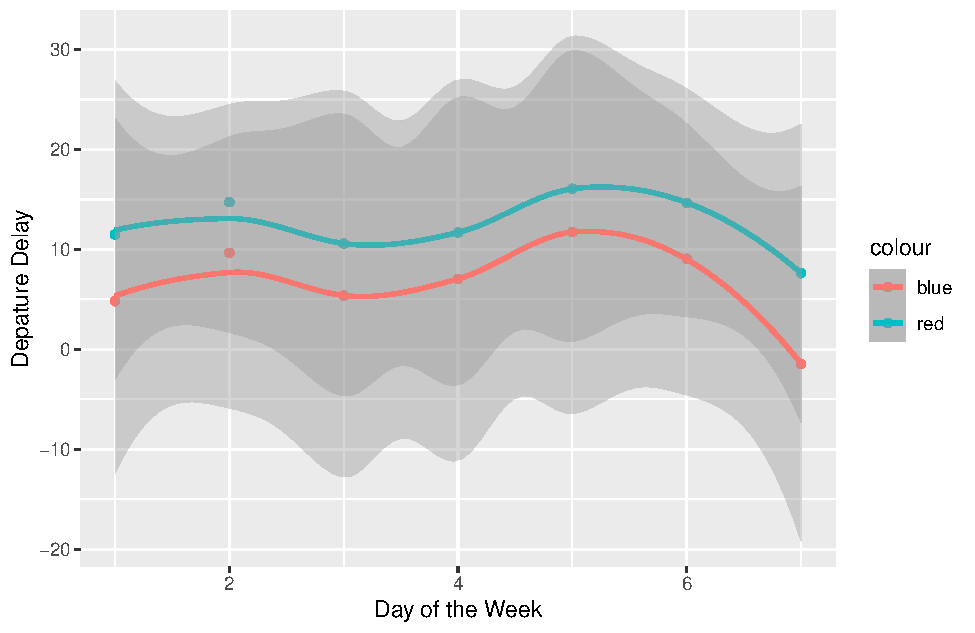
\includegraphics{Midterm.sa_files/figure-latex/unnamed-chunk-7-1.pdf}

\begin{Shaded}
\begin{Highlighting}[]
\CommentTok{\# Saturdays look like the bast day to leave if you are minimizing delays. This is due to lower average delays and even average arriving early on Saturdays.}
\end{Highlighting}
\end{Shaded}

\hypertarget{exercise-6-10-pts}{%
\subsubsection{(6) 16.3.4 Exercise 6 (10 pts)}\label{exercise-6-10-pts}}

What makes the distribution of \texttt{diamonds\$carat} and
\texttt{flights\$sched\_dep\_time} similar?

\begin{Shaded}
\begin{Highlighting}[]
\CommentTok{\# Not going to lie, it took me a while to figure out this problem but it makes so much sense now.}

\FunctionTok{ggplot}\NormalTok{(diamonds, }\FunctionTok{aes}\NormalTok{(}\AttributeTok{x =}\NormalTok{ carat)) }\SpecialCharTok{+}
  \FunctionTok{geom\_histogram}\NormalTok{(}\AttributeTok{binwidth =}\NormalTok{ .}\DecValTok{05}\NormalTok{) }\SpecialCharTok{+} 
  \FunctionTok{labs}\NormalTok{(}\AttributeTok{y =} \StringTok{"Count"}\NormalTok{,}\AttributeTok{x =} \StringTok{"Carat"}\NormalTok{)}
\end{Highlighting}
\end{Shaded}

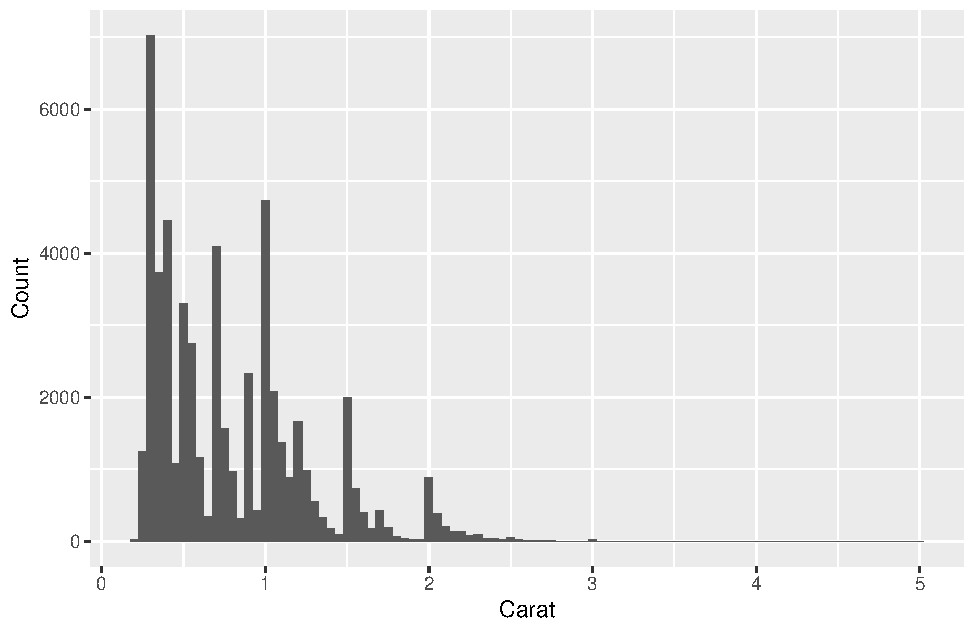
\includegraphics{Midterm.sa_files/figure-latex/unnamed-chunk-8-1.pdf}

\begin{Shaded}
\begin{Highlighting}[]
\FunctionTok{ggplot}\NormalTok{(flights\_fixed, }\FunctionTok{aes}\NormalTok{(}\AttributeTok{x =} \FunctionTok{minute}\NormalTok{(sched\_dep\_time))) }\SpecialCharTok{+}
  \FunctionTok{geom\_histogram}\NormalTok{(}\AttributeTok{binwidth =} \DecValTok{1}\NormalTok{)}\SpecialCharTok{+}
  \FunctionTok{labs}\NormalTok{(}\AttributeTok{y =} \StringTok{"Count"}\NormalTok{,}\AttributeTok{x =} \StringTok{"Scheduled Depature Times"}\NormalTok{)}
\end{Highlighting}
\end{Shaded}

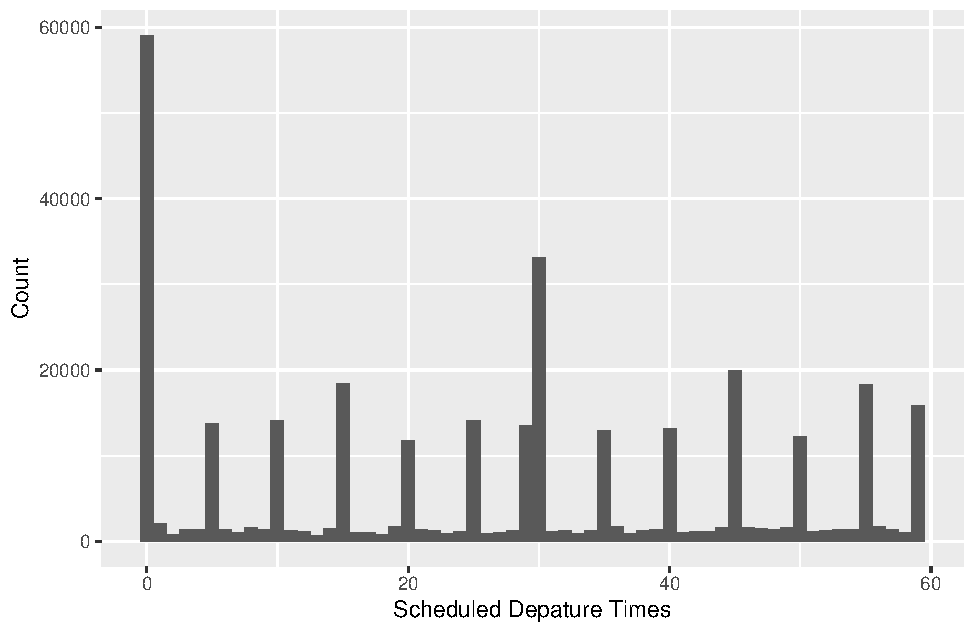
\includegraphics{Midterm.sa_files/figure-latex/unnamed-chunk-8-2.pdf}

\begin{Shaded}
\begin{Highlighting}[]
\CommentTok{\# Looking at the two graphs, it is easy to see that both distributions of data have spikes. This is due to the nature of both data sets. Where each sculptor for the diamond has a goal for the size of diamond and wants no less than a whole number carat. The same way the flights want to leave in minutes ending in 5 or 0 since it is easier for people to understand.}
\end{Highlighting}
\end{Shaded}


\end{document}
